\documentclass[10pt,letterpaper]{article}

\usepackage{cogsci}
\usepackage{pslatex}
\usepackage[nodoi]{apacite}
\usepackage{amsmath, amssymb}
\usepackage{graphicx}
\usepackage{caption}
\usepackage{subcaption}
\usepackage{tabulary}
\usepackage{multirow}
\usepackage{rotating}
\usepackage{times}
\usepackage{csquotes}
\usepackage{calc}
\usepackage{verbatim}
\usepackage[bottom]{footmisc}
\usepackage[font=footnotesize,skip=2pt]{caption} 



\title{One-shot compositional function learning}
 
\author{\textbf{Pablo Le\'on-Villagr\'a$^1,$ Eric Schulz$^2$, Maarten Speekenbrink$^2$, Samuel J. Gershman$^3$ \& Christopher G. Lucas$^1$}\medskip\\ 
$^1$School of Informatics, University of Edinburgh\\
$^2$Department of Experimental Psychology, University College London\\
$^3$Department of Psychology and Center for Brain Science, Harvard University}

\usepackage[textsize = tiny]{todonotes}
\setlength{\marginparwidth}{1.5cm} 
\newcommand{\mtodo}[2][]
{\todo[caption={#2}, size=\small, #1, color = green, inline]{\renewcommand{\baselinestretch}{1}\selectfont \textbf{MS}: #2}~}
\newcommand{\smtodo}[2][]
{\todo[size=\footnotesize, color = green, #1]{#2}~}%Remove me again once Maarten's comments resolved


\begin{document}

\maketitle
\begin{abstract}
We explore the human ability to discover and generalize compositional rules in the domain of function learning. Across four experiments we find evidence that participants are able to identify compositional functions and, if the individual components are distinguishable, perform one-shot generalization of the compositional rule. We propose that the ability to detect and memorize compositional rules and components is crucial to the human ability to perform one-shot generalization.

\textbf{Keywords:} 
Rule discovery; Compositionality; Gaussian processes; Function learning; Generalization
\end{abstract}

\section{Introduction}

People have an impressive ability to learn from sparse data \cite{tenenbaum2011grow}. Presented with only one example of a concept, even children can generalize far beyond the encountered data \cite{perfors2009learning}. Some researchers have proposed that this ability to generalize from sparse data is a core ingredient of intelligence \cite{lake2016building}. What is the source of this ability?

One source of strong generalization is compositionality: by discovering the building blocks of concepts and the composition rules that combine them to form more complex concepts, the same building blocks can be composed to make predictions about novel concepts. For example, words can be composed into an infinite variety of sentences, and parts can be composed into an infinite variety of objects \cite{kemp2012exploring, dechter2013bootstrap,lake2015human}. 

The goal of the work reported here is to understand how compositional structure can aid one-shot generalization in human function learning. While function learning has been studied extensively \cite{mcdaniel2005conceptual}, little is known about the human limits of generalization from sparse data.%We propose that participants progressively build up a library of composition rules (e.g., addition and multiplication) and building blocks (e.g., lines and sinusoids) for a given domain, and then use these elements to decompose new functions.

Imagine you are trying to book an accommodation ahead of a conference in an expensive city. You know that the rental prices fluctuate according to certain temporal patterns (e.g., prices normally increase as the rental date approaches). Moreover, there might be some fluctuations from day to day such that it could be more expensive to book a place on a Sunday when everyone is looking up accommodations than on a Tuesday when most people are at work. These patterns may compose in different ways---for example, additively or multiplicatively. Jointly learning the patterns and their compositional structure allows you to make a rich variety of predictions about new patterns; if you are shown two new patterns (e.g., declining prices and sinuosoidal seasonal fluctuations), you can infer what their composition will look like.

We use a Gaussian process regression framework to assess how participants make generalizations about compositional functions. Gaussian process regression is a non-parametric Bayesian approach to regression problems, and has recently been found to describe human function learning across a variety of experiments well \cite{lucas2015rational, griffiths2009modeling}. Moreover, as Gaussian processes utilize a kernel to encode assumptions about functional structure, and kernels can be combined to describe complex patterns, the framework has been used to develop a compositional theory of intuitive functions~\cite{schulz2016compositional, villagrahuman}.

Across four experiments asking participants to reason about combinations of functions, we found evidence for efficient generalization from sparse data, even in a one-shot learning scenario. This ability depended crucially on the distinguishability of the composition rules as well as on the salience of the component patterns.

\section{Gaussian process regression as a theory of compositional function learning}

%SG: the paragraphs below are (a) partially redundant with the previous section, and (b) not very informative about what we're actually doing. I think it would be more useful to review the work on function learning that we're building on. This is what I've done.

%Compositionality is the notion that complex structure is made of simpler elements. These simple elements constitute as primitives that can be combined to create more complex elements that can also be re-combined, and so forth \cite{fodor1975language}. We will refer to the rules by which compositional elements can be combined as \emph{compositional operators}. 

%The idea that the mind constructs more complex explanations from a simple set of primitives has a longstanding tradition within the cognitive science community. Therein, compositionality has largely been studied within rule-based concept learning paradigms in which the compositional building blocks are defined as logical primitives and participants' errors within reasoning tasks are used to infer the rules they apply \cite{bruner1956austin, shepard1961learning}. 

%The rich tradition of findings supporting a compositional view of cognition lead to the argument that compositionality is an important prerequisite for designing algorithms ``that learn and think like people'' \cite{lake2016building}. However, if we want to take this argument seriously and indeed benchmark machine learning algorithms against ``human-like'' compositional thought, then what we need is a psychologically plausible theory of how people actual reason about and generalize from compositional rules.% In particular, a valid theory of human compositional rule learning should start by mapping out the conditions under which compositional rules can be learned from sparse data. This will be the goal of this paper.
%P: I don't think we do this

Our work builds on a recent theory of function learning \cite{lucas2015rational}, according to which people compute a posterior over functions by applying Bayes' rule:
\begin{align}
p(f|\mathcal{D}) \propto p(\mathcal{D}|f) p(f),
\end{align}
where $f: \mathcal{X} \mapsto \mathbb{R}$ is a function over some input space $\mathcal{X}$, and $\mathcal{D} = \{\mathbf{x}_n,y_n\}_{n=1}^N$ is a collection of input-output pairs. The likelihood $p(\mathcal{D}|f)$ measures how well the function fits the data, and the prior $p(f)$ specifies the inductive bias over functions. For example, evidence suggests that humans have an inductive bias favoring linear functions with a positive slope \cite{brehmer1974hypotheses,kalish2007iterated}.

A Gaussian process is an expressive and analytically convenient prior over functions \cite{rasmussen2006gaussian}. One can use a Gaussian process to define inductive biases for linear, periodic, non-stationary functions, as well as for many different forms of smoothness. Bayesian inference with Gaussian processes admits closed-form expressions, and is closely related to both rule-based and similarity-based frameworks for function learning \cite{lucas2015rational}. Because the mathematical details are not central to the present work, we refer the reader to the above references for more information.

Importantly, Gaussian processes can be composed to build models for more complex functions. This has proven to be a successful approach in machine learning \cite{duvenaud2013structure}, and recently we have shown how the same framework can be used to understand how humans model complex functions \cite{schulz2016compositional, villagrahuman}. Compositional Gaussian processes predicted human interpolation and extrapolation performance better than an equally expressive non-compositional model. Furthermore, we showed that compositionality affects performance on a variety of other tasks involving mental representations of functions, such as short-term memory, numerosity judgements, and change detection. Here, we build on this work by showing that compositionality supports one-shot discovery of functional structure.

%We use Gaussian process regression as a general framework to approach compositionality for functional relationships. In a Gaussian process, kernels can be added and multiplied together to create new kernels, allowing the creation of richly structured models from established base components \cite{duvenaud2013structure}. This in turn provides a powerful framework to model complex data as made of simpler parts and has recently been used to assess participants' structural inductive biases across a diverse set of cognitive domains \cite{schulz2016compositional, villagrahuman}. Here, instead of focusing on structural inductive biases, we are interested in the compositional operators that participants might be able to learn. More specifically, the question we are trying to address is whether and how participants can extract compositional operators from single examples and generalize these operations to subsequent scenarios.

\section{Experimental paradigm}\label{sec:osetup}

In Experiments 1-3, participants were asked to make judgements about sales patterns produced by fictitious alien plants on the intergalactic market. They were first shown the sales pattern over time for a Plant A and for a Plant B. These sales patterns, $f_A$ and $f_B$, were functions sampled from a Gaussian process parametrized by kernels $k_A$ and $k_B$ respectively. Afterwards, participants were shown the sales pattern for a new plant which was an offspring of plant A and B. The sales pattern for the offspring plant, $f_{\text{offspring}}$, was a sample from a Gaussian process with a kernel $k_{\text{offspring}}$ which had been generated by applying a compositional operator $g$ to the two base kernels (the parents), i.e. $k_{\text{offspring}}=g(k_A,k_B)$. The sampled functions $f_A$, $f_B$, and $f_{\text{offspring}}$ constituted the \emph{learning set}.

Afterwards, participants were shown sales pattern $f_C$ for a Plant C and sales pattern $f_D$ for a Plant D. The patterns $f_C$ and $f_D$ were samples from Gaussian processes with kernels $k_C$ and $k_D$ (which could differ from kernels $k_A$ and $k_B$). The sampled functions $f_C$ and $f_D$ constituted as the \emph{test set}. Participants were then asked to judge what the sales pattern $f_{\text{new offspring}}$ of the offspring might look like, given that this new plant is the offspring of plant C and D. If participants detect the compositional rule generating the offspring in the learning set and generalize to the test set, the sales pattern for the new offspring should involve the same compositional rule. This pattern $f_{\text{new offspring}}$ would be a sample from a Gaussian process with a kernel $k_{\text{new offspring}}$ which is generated by applying the same compositional rule $g$ to kernels $k_C$ and $k_D$, i.e. $k_{\text{new offspring}} = g(k_C,k_D)$. We will refer to the function corresponding to this composition as the \textit{true function} throughout this paper. 
For an example of the set-up used in the experiments, see Figure~\ref{fig:setupEx}.


\begin{figure}[ht!]
\centering
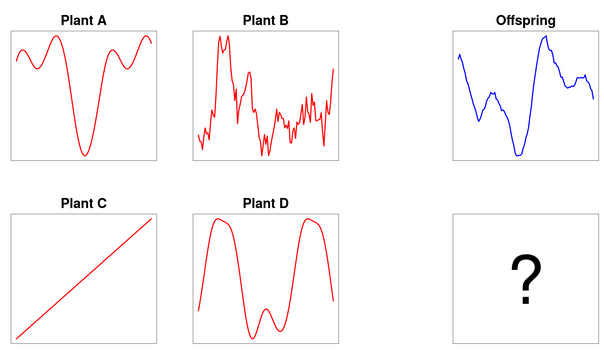
\includegraphics[width=0.45\textwidth]{screenshot1.png}
\caption{\textbf{Setup for Experiments 1-3}.
Participants were first presented sales patterns for two plants (A,B) and the sales pattern of their offspring. Sales patterns were sampled from a Gaussian process - In this example sales patterns for plant A are generated by a periodic kernel, sales patterns for plant B from a Ornstein-Uhlenbeck kernel and the offspring of A and B from the sum of the kernels A and B. Given this training set, participants were then presented sales patterns for 2 more plants (C, D) and had to infer the sales pattern of their potential offspring. Plant C and D constituted the test set. In this example the sales pattern for plant C is generated from a linear kernel and the pattern for plant D is generated by a periodic kernel. If participants generalize the compositional rule generating the offspring in the training set, the offspring of C and D should be a sample from a kernel composed from the sum of the linear and periodic kernel.}
\label{fig:setupEx}
\end{figure}

\subsection{Generating Functions}\label{ssec:genfun}

The sales patterns were functions sampled from a Gaussian process $$f_i \sim \mathcal{GP}(\mu, k_i(\mathbf{x},\mathbf{x'})),$$ where the mean $\mu$ was zero and the covariance kernel $k_i$ was sampled from the set of \textit{base kernels} or a composition of those.

The base kernels used in Experiments 1 and 2 were the radial basis function kernel (RBF)
\begin{align}
k_{\text{RBF}}(\mathbf{x},\mathbf{x}')=\theta_1^2\exp\left(-\frac{(\mathbf{x}-\mathbf{x}')^2}{2\theta_2^2}\right)
\end{align}
with $\theta_1=1$ and a length-scale of $\theta_2=0.1$, the linear kernel
\begin{align}
k_{\text{LIN}}(\mathbf{x},\mathbf{x}')=\theta_3(\mathbf{x}-\theta_4)(\mathbf{x}'-\theta_4)
\end{align}
with $\theta_3=1$ and $\theta_4=2$, and a periodic kernel
\begin{align}
k_{\text{PER}}(\mathbf{x},\mathbf{x}')=\theta_5^2\exp\left(-\frac{2\sin^2(\pi|\mathbf{x}-\mathbf{x}'|\theta_6)}{\theta_{7}^2}\right)
\end{align}
with $\theta_{\{5,6\}}=1$ and $\theta_{7}=0.2$. In Experiment 3 and 4, instead of the RBF-kernel, we used an Ornstein-Uhlenbeck kernel (ORU)
\begin{align}
k_{\text{ORU}}(\mathbf{x},\mathbf{x}')=\theta_8^2\exp\left(-\frac{|\mathbf{x}-\mathbf{x}'|}{2\theta_9^2}\right)
\end{align}
with $\theta_8=1$ and $\theta_9=3$.

The two assessed compositions were the \emph{Addition}, $+$, and \emph{Multiplication}, $\times$, of two kernels. See Figure~\ref{fig:compex} for samples resulting from adding or multiplying kernel functions from our base kernels.

\begin{figure}[ht!]
\centering
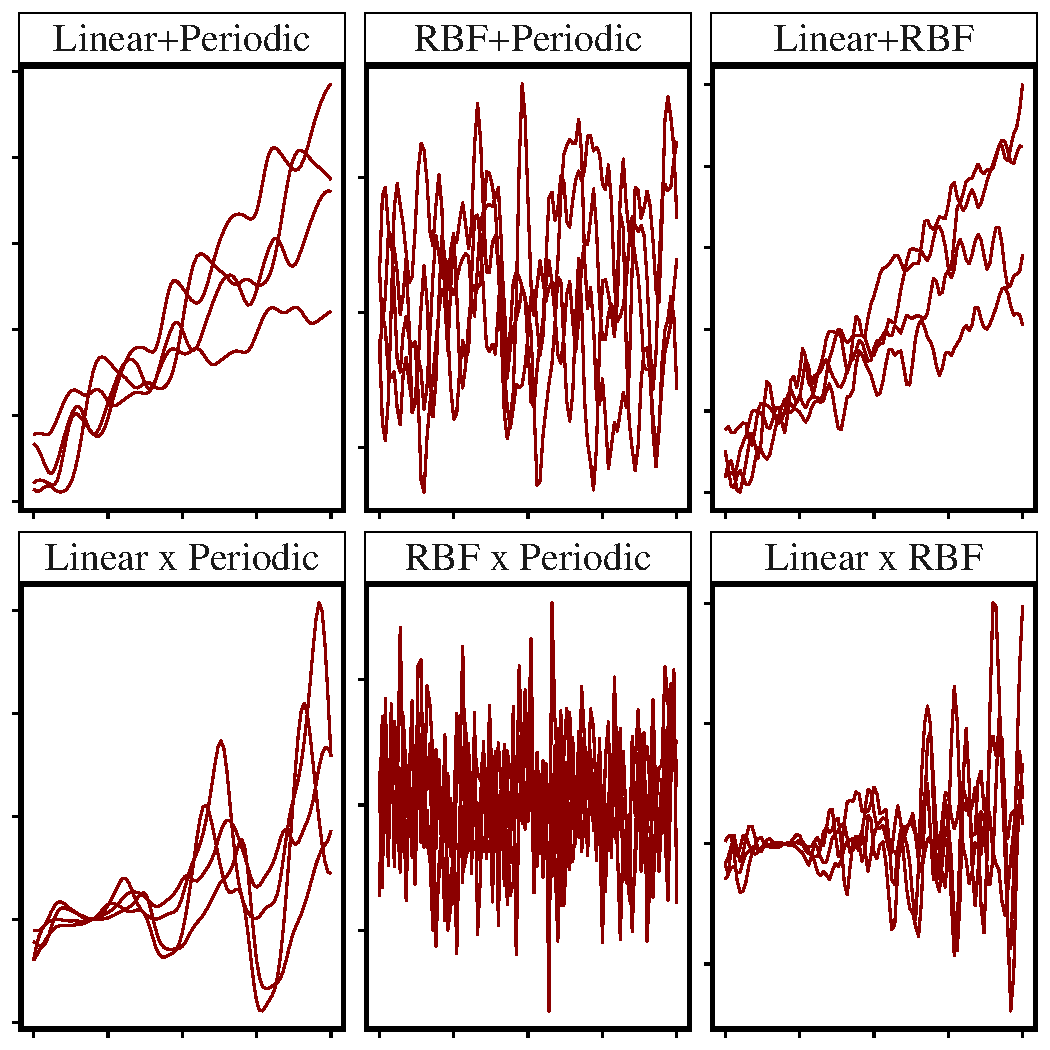
\includegraphics[width=0.42\textwidth]{compexamples.pdf}
\caption{\textbf{Samples from GPs with composed kernels} Samples from a composed kernel resulting from adding a linear and a periodic kernel exhibit a linear trend with periodicity. Adding a periodic to a RBF kernel adds periodicity to smooth functions, whereas adding a linear to a RBF kernel leads to smooth functions with a linear trend. Linear $\times$ Periodic leads to periodicity with increasing amplitude, whereas RBF$\times$ periodic generates samples that are locally periodic. Linear $\times$ RBF leads to smooth functions with increasing amplitude.}
\label{fig:compex}
\end{figure}


\section{Experiment 1: Distinguishing compositional rules}
The first experiment assessed if participants can successfully identify a previously encountered composition from its single-kernel components and the alternative composition.

\subsection{Participants}
50 participants were recruited online through Amazon's Mechanical Turk web service. Participants had an mean age of M$_\text{age}=31.02\pm6.84$, and 16 of them were female. Participants received \$0.3 for their participation. 

\subsection{Design}
Functions were sampled within $\mathbf{x}=[0,0.1,\dots,10]$ from the 3 base kernels as specified in the section on generating functions~\ref{ssec:genfun}. On every trial, 2 of the 3 kernels were sampled without replacement and one composition rule ($+$ or $\times$) was chosen at random. The learning set consisted of one function sampled from the first kernel, one function sampled from the second kernel, and one sampled from the composed kernel. In the test set, participants again saw one function sampled from each of the two kernels and then had to choose the most likely composition of the two kernels from a set of options. The 4 proposed options were samples from the true composition, an alternative composition (for example, $\times$ if the true composition was $+$), and the two base kernels that generated the functions.

\subsection{Procedure}
Participants were told that they had to make judgments about sales patterns of different fictitious alien plants on the intergalactic market. First, they were shown patterns from two different plants and their offspring. They were told that the x-axis marked the days over which a plant was traded and that the y-axis showed how well it sold on a particular day. Finally, sales patterns for two new plants were shown and participants had to choose the sales pattern of their potential offspring. After a full example trial, participants were presented with 10 trials and told that they should treat every trial as new.
 
\subsection{Results}

Participants selected the sales pattern generated by the true composition significantly more often than the pattern generated by the alternative composition ($t(49)=5.11$, $p<0.001$), or the other two base kernels ($t(49)=6.99$, $p<0.001$). In addition, participants also selected the alternative composition significantly more often than the samples from the base kernels ($t(49)=2.95$, $p<0.01$), showing a tendency to prefer compositional over non-compositional samples. There was no significant preference for additive compositions over multiplicative ones ($t(102)=0.11$, $p>0.91$). Additive compositions were as likely to be identified correctly  as multiplicative compositions ($t(102)=0.83$, $p>0.4$). Figure~\ref{fig:results1} shows the proportion of choices averaged over all participants.
\begin{figure}[ht!]
\centering
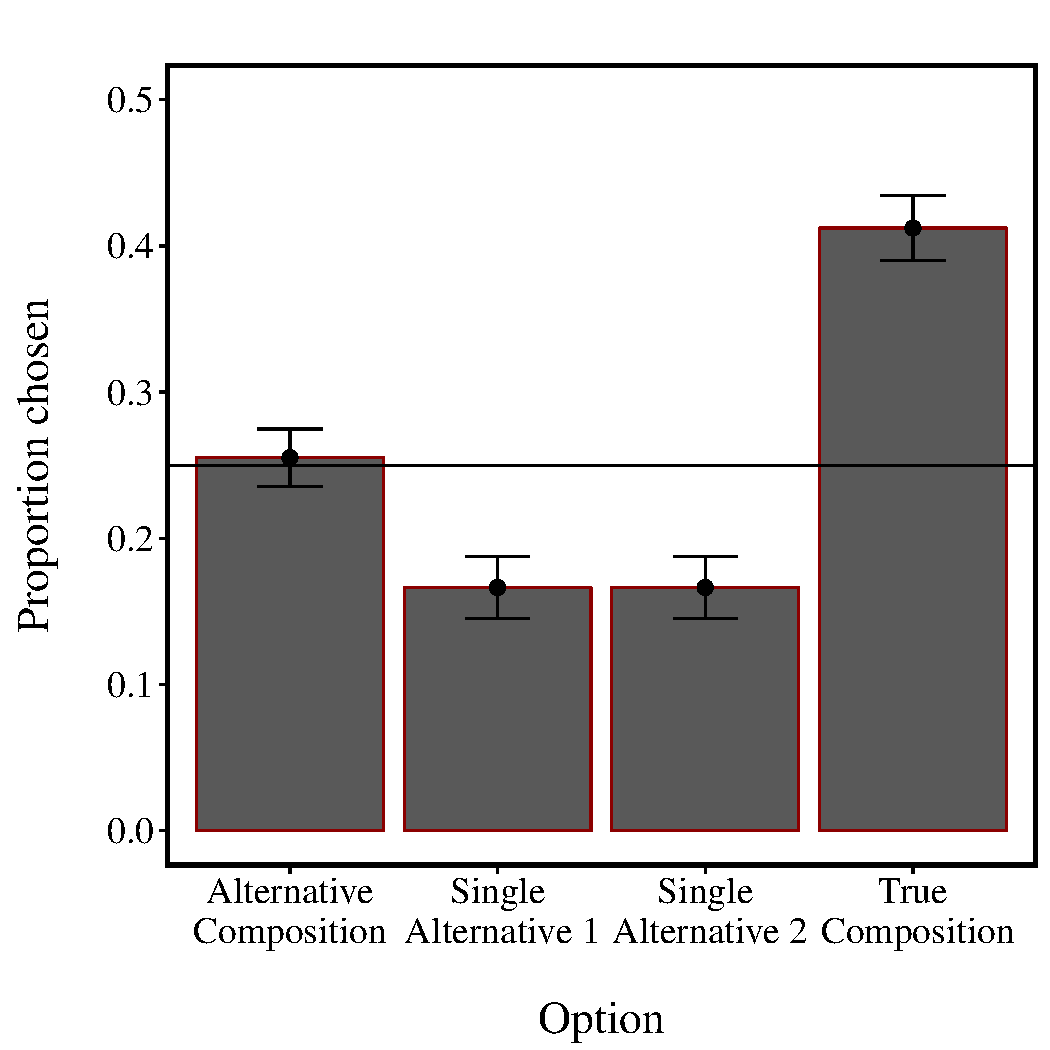
\includegraphics[width=0.4\textwidth]{results1.pdf}
\caption{\textbf{Chosen sales patterns for Experiment 1}. Participants preferred samples generated from compositions of kernels over base kernel alternatives. Additionally, they selected the true composition significantly more often than the alternative composition. The horizontal line indicates chance level. Error bars represent the standard error of the mean.}
\label{fig:results1}
\end{figure}

Comparing the different kernel combinations, we found that trials involving compositions of a RBF and a periodic kernel were significantly more difficult than trials involving any other combination ($t(151)=-3.5$, $p<0.001$), independent of the compositional rule. Additionally, none of the base kernels led to a significant decrease in correct responses (all $p>0.2$).

Overall, Experiment 1 showed that participants were able to detect the correct composition rule. Participants also preferred the alternative composition over base kernel samples, indicating a sensitivity for compositionality in general. Finally, there is some indication that kernel compositions involving RBF and periodic kernels are more difficult to distinguish than others. 
While participants detected and preferred the true compositions in Experiment 1, this does not provide enough evidence for one-shot compositional rule generalization, as the test and training set corresponded to the same type of base kernels and compositional rule.

\section{Experiment 2: One-shot rule generalization}
In Experiment 2 we tested, if participants can generalize the compositional rule from the test set to a composition involving a novel component.

\subsection{Participants}
50 participants were recruited online through Amazon's Mechanical Turk web service. Participants had a mean age of M$_\text{age}=30.5\pm 7.04$. 19 participants were female. They received \$0.3 for their participation. 

\subsection{Design \& Procedure}
The design and procedure corresponded to Experiment 1 with one crucial difference - instead of presenting the same 2 base kernels in the learning and test set, one of the base kernels in the test set was replaced with the remaining kernel in the set of base kernels (e.g. if the training consisted of the RBF and linear kernel the test set consisted of the RBF and periodic).

\subsection{Results}

As in Experiment 1, participant selected the sales pattern generated by the true composition significantly more often than samples from the two base kernels ($t(49)=4.66$, $p<0.001$). However, the alternative composition was chosen as frequently as the true composition ($t(49)=0.66$, $p>0.5$). Similar to the results in Experiment 1, participants were less likely to select the true composition if the test set included samples generated by the RBF kernel, as compared to the other kernels ($t(153) = -2.196$, $p<0.05$). For the proportion of choices averaged over participants, see Figure~\ref{fig:results2}.
\begin{figure}[ht!]
\centering
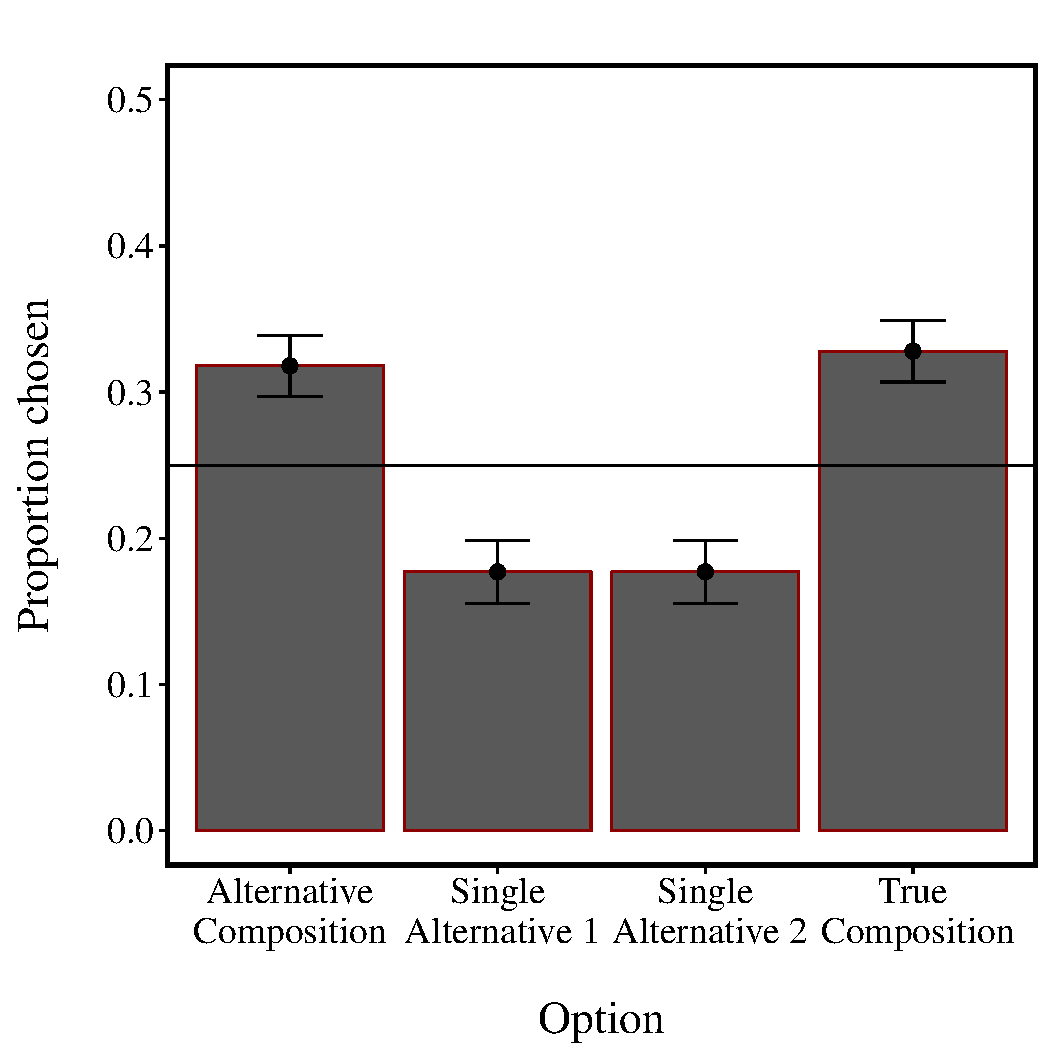
\includegraphics[width=0.4\textwidth]{results2.pdf}
\caption{\textbf{Chosen sales patterns for Experiment 2}. Participants preferred samples generated from compositions of kernels over base kernel alternatives. However, they did not distinguish between the two alternative compositions. The horizontal line indicates chance level. Error bars represent the standard error of the mean.}
\label{fig:results2}
\end{figure}



%P:
%rbf problematic as single kernel or as composition?
%what about preference for additive compositions over multiplicative ones
%what about additive compositions more likely to be identified correctly
%ES: I had some further tests on that in there, but someone (Chris? Maarten?) said it looked like we were fishing for results.
%ES2: To make it a little clearer, in the first experiment, periodic and rbf together were bad, in the second rbf alone was the culprit.

%P: so all cases in which rbf features on the second row? as the proposed functions are the single kernel samples of the test-set compositons plus the 2 compositons
%If this is correct - we should rewrite it stating that they were worse if the rbf was in the test set than when the rbf was in the training set, which is in concordance with the difficulty faced in experiment1 

\section{Interim Discussion}
Experiment 1 showed that participants generally preferred compositional rules and could distinguish the true composition from the alternative. However, when the test set contained a novel component, participants could not distinguish between the additive and multiplicative rule in Experiment 2. These results challenge the idea that participants generalize the composition rule to new instances. However, in both Experiment 1 and 2, trials involving the RBF kernel in the test set were harder to identify. This suggests that the inability to discriminate between the true and the alternative composition could result from a difficulty in discriminating RBF-composition rules.
In Experiment 3 we tested this hypothesis, replacing the RBF-kernel with a more distinctive kernel - the Ornstein-Uhlenbeck kernel (ORU). Samples from an ORU-kernel are a less smooth than samples from the RBF kernel and therefore might be easier to distinguish empirically. For a comparison of samples from a ORU, RBF and periodic, see Figure~\ref{fig:rbforu}.

%CL: I don't understand why introducing the new kernel would have the effect of eliminating the abilitity to distinguish between the true composition and the alternative.

%@SAM: if we want to make a claim about the ORU, then maybe here would be the right place?
%
%What makes ORU better than RBF here: less similar to periodic?

\begin{figure}[ht!]
\centering
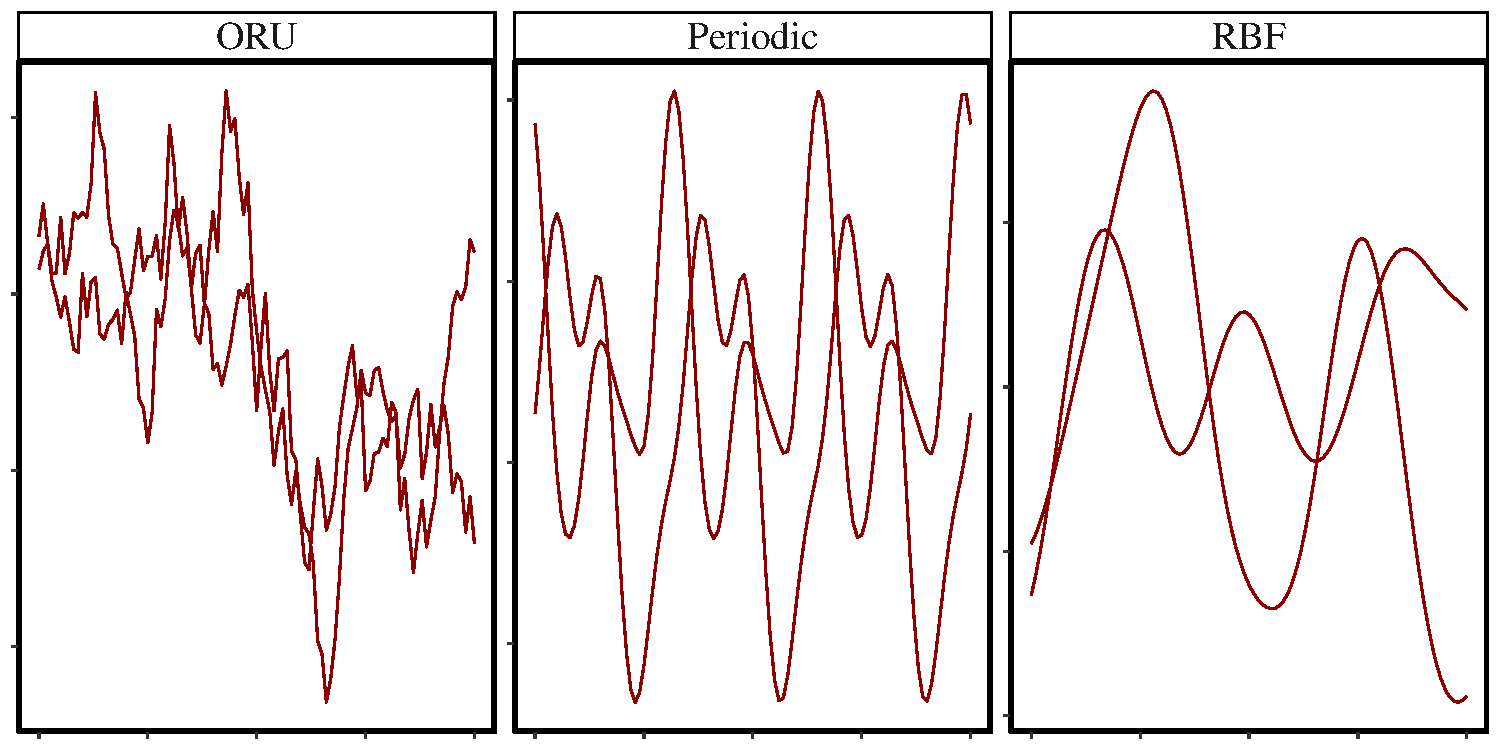
\includegraphics[width=0.49\textwidth]{oruexamples.pdf}
\caption{\textbf{Samples from Ornstein-Uhlenbeck, periodic, and radial basis function kernel}. RBF and periodic kernels look more similar to each other than samples from Ornstein-Uhlenbeck.}
\label{fig:rbforu}
\end{figure}


\section{Experiment 3: One-shot rule generalization with distinguishable components}

\subsection{Participants}
50 participants were recruited online through Amazon's Mechanical Turk web service. Participants had a mean age of M$_\text{age}=32.54 \pm 9.58$, and 20 of them were female. Participants were paid \$0.3 for their participation. 

\subsection{Design and Procedure}
In Experiment 3 the RBF kernel was substituted with an ORU-kernel. Otherwise, design and procedure were the same as in Experiment 2.

\subsection{Results}
As in Experiments 1 and 2, participants chose the true and the alternative composition significantly more often than samples from the base kernels ($t(40)= 6.13$, $p<0.001$, $t(49)=4.53$, $p<0.001$). More importantly, participants selected the true composition significantly more often than the alternative ($t(49)= 2.43$, $p<0.05$). % even when only analyzing participants' responses on the very first trial ($t(49)=2.29$,$p<0.05$). P: This is great, but we don't really talk about it much and we would have to contrast this with performance in the first trial in all other experiments? I would not report this.
For the average choice proportions, see Figure~\ref{fig:results3}.
\begin{figure}[ht!]
\centering
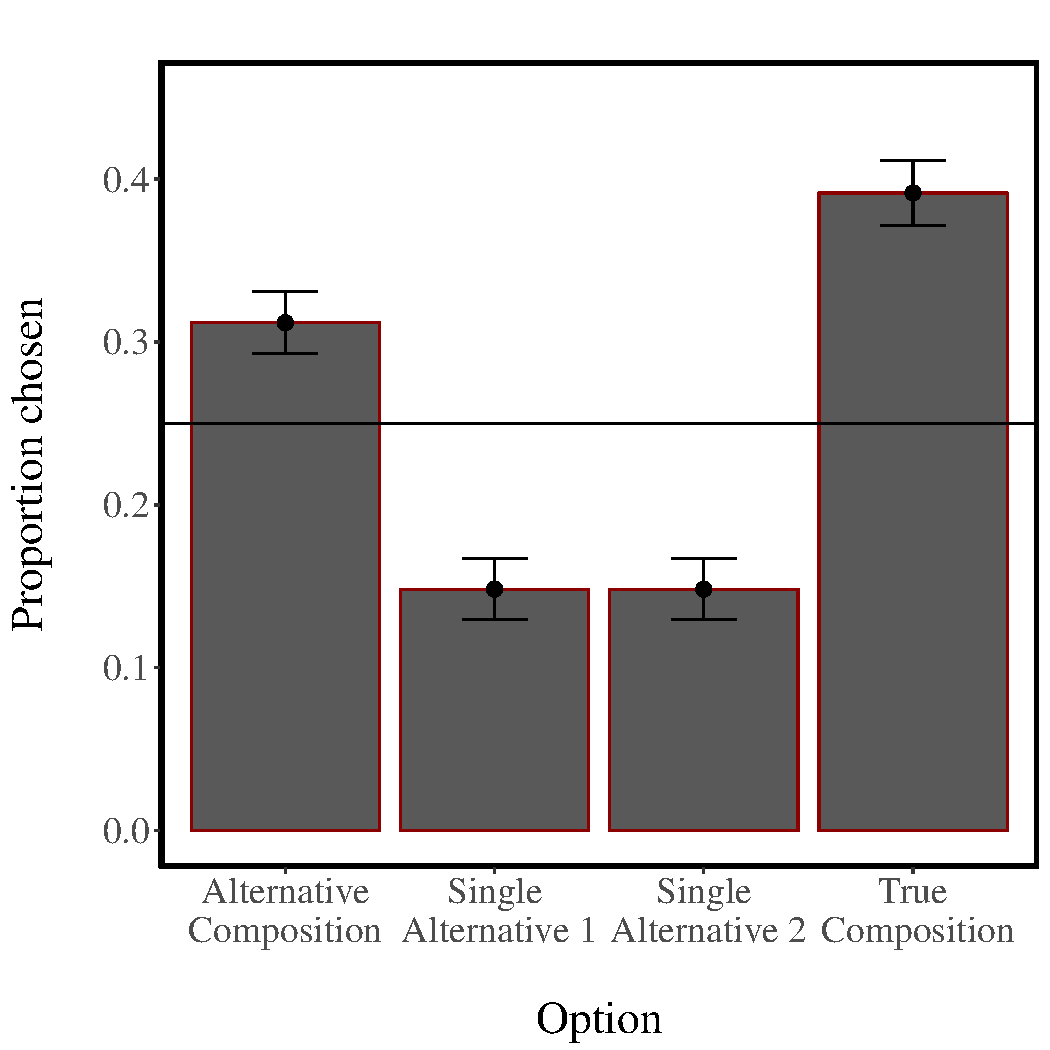
\includegraphics[width=0.4\textwidth]{results3.pdf}
\caption{\textbf{Chosen sales patterns for Experiment 3}. Again, participants preferred samples generated from compositions of kernels over base kernel alternatives. Additionally, they selected the true composition significantly more often than the alternative composition. The horizontal line indicates chance level. Error bars represent the standard error of the mean.}
\label{fig:results3}
\end{figure}

Additionally, the number of correct responses did not differ for trials involving the ORU-kernel ($t(173)=-1.27$, $p>0.2$), nor for samples from the composition of a ORU and periodic kernel ($t(171)=-0.64$, $p>0.5$).
%This can also be seen when assessing the effect of different kernel-combinations onto participants' responses, which showed that --contrary to the findings about the RBF kernel in Experiment 1 and 2-- there was no effect of the Ornstein-Uhlenbeck kernel on participants' average correct responses ($t(173)=-1.27$, $p>0.2$). There was also no effect of compositions involving both an Ornstein-Uhlenbeck and a periodic kernel on participant's average of correct response ($t(171)=-0.64$, $p>0.5$).


The results of Experiment 3 validate our hypothesis that the failure to perform one-shot generalization in Experiment 2 resulted from the difficulty of generalizing a compositional rule involving the RBF-kernel. Substituting the RBF-kernel with a more salient ORU-kernel, we found that participants can generalize the compositional rule and managed to distinguish between additive and multiplicative compositions. 

\section{Experiment 4: Alternative explanations}

Experiments 1-3 showed that participants can perform one-shot rule generalization given only one example of a composition. However, this ability to generalize the correct composition depended on the distinctiveness of the samples generated by the base kernels and the composition of kernels. 
Given this interdependence, one natural alternative explanation for the participants' ability to infer the true composition is that instead of detecting the compositional rule in the learning set and generalizing to the test set, participants simply matched the offspring in the training set to the presented samples, based on surface features (for example local variance or monotonicity).
Experiment 4 assessed whether the true composition could be detected solely based on surface features of the offspring in the training set.


\subsection{Participants} 
50 participants were recruited online through Amazon's Mechanical Turk web service. Participants had a mean age of M$_\text{age}=32.83 \pm 10.63$, and 20 of them were female. Participants received \$0.3 for their participation. 

\subsection{Design and Procedure}
The design and procedure was the same as in Experiment 3 with one crucial difference - participants did not see any samples of the base kernels (i.e. they did not see two base kernels, but only the composition in the training and did not see any base samples in the test set). Participants were instructed to imagine the rules by which the sample in the training set was produced and then pick the pattern that they thought was most likely created by applying the same rule.

\subsection{Results}

Even though participants exhibited a small tendency to choose the true composition over the alternative, this difference was not significant ($t(49)$=1.7, $p>0.05$). Moreover, participants did not choose the true composition more frequently than any of the samples generated by a base kernel ($t(49)= 1.29$, $p>0.2$) and none of the patterns were chosen significantly more often than chance (all $p>0.1$).
Figure~\ref{fig:results4} shows the average choice proportions.
\begin{figure}[ht!]
\centering
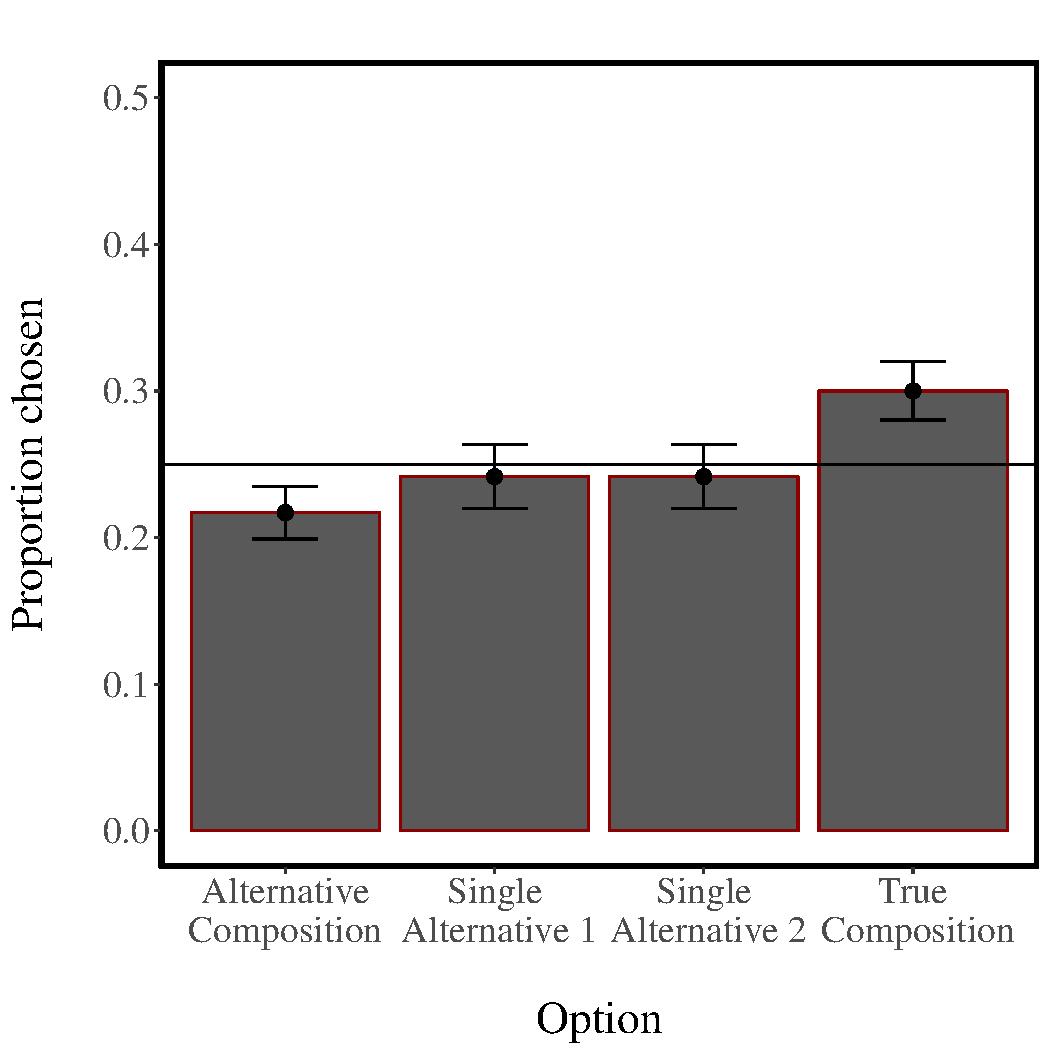
\includegraphics[width=0.4\textwidth]{results4.pdf}
\caption{\textbf{Chosen sales patterns for Experiment 4}. Participants did not prefer samples generated from compositions of kernels over base kernel alternatives, nor did they select the true composition over the alternative. The horizontal line indicates chance level. Error bars represent the standard error of the mean.}
\label{fig:results4}
\end{figure}
 
 
\section{Discussion and Conclusion}

We explored the human ability to discover and generalize compositional rules in the domain of one shot function learning. Experiment 1 showed that people are able to learn and distinguish compositions from simpler generating functions, as well as alternative compositions, if the types of generating functions in the training are the same as in the test set. The second experiment assessed a full version of one-shot rule generalization and found that, while participants were able to detect samples generated by compositions, they were unable to distinguish between addition and multiplication. However, replacing the RBF-kernel with the more distinctive ORU-kernel, we found that participants were able to infer the true compositional rule. Finally, when the training set did not contain the individual components, participants were unable to identify the true composition. Therefore, we can conclude that the ability to select the true composition rests fundamentally on learning the individual components, as well as the compositional rule, and cannot be explained by simply matching samples based on surface similarity. This constitutes a first existence proof of one-shot compositional function learning in humans.

We have proposed that the ability to perform one-shot generalization requires that people detect compositional patterns and memorize the components as well as the compositional rules. These memorized components and rules allow for flexible reuse of compositions and thereby can lead to rapid model building, even in novel situations. However, this ability seems to depend on the discriminability of the components and their compositions.

Future studies could try to assess factors influencing the ability to generalize compositional rules. For example, biases over compositional operators might in fact track real-world statistics \cite{griffiths2006optimal}. If real-world sales patterns are more likely to be composed in additive instead of  multiplicative fashion, a bias towards additive compositions might be useful and rational. 

Another avenue for future research could be to formalize the way in which participants internally hypothesize and assess different components. Indeed, one of the first psychological theories of function learning proposed that people employ a hierarchy of different parametric functions that they test and adapt whenever the data contradict their internal representation \cite{brehmer1974hypotheses}. Such an iterative approach of testing and expanding compositional components would fit rather well with the greedy search algorithms underpinning recent models of compositional structure search \cite{duvenaud2013structure} and may suggest novel models and experimental ideas for human, as well as artificial, compositional function learning and generalization.

\section{Acknowledgments}
PLV and ES contributed equally. PLV is supported by the ILCC, School of Informatics Edinburgh. ES is supported by the UK Centre for Financial Computing and Data Analytics.
\bibliographystyle{apacite}
\setlength{\bibleftmargin}{.125in}
\setlength{\bibindent}{-\bibleftmargin}

\bibliography{references}
\end{document}